\section{\label{sec:kbpo:kbpo} Implementing on-demand evaluation as an online service}

\pl{a lot of this section doesn't seem like it has to do with the online service part,
but talking about the sampling distribution that even defines what the evaluation metric is;
I think this needs to be more clearly it's own section labeled 'sampling distribution' or something,
and made clear that while most of this thesis is focusing on improving the statistical efficiency of estimation,
this is about what we're estimating.
}

\pl{also, this discussion is pretty in the weeds of KBP;
I'd add a paragraph saying how this is a general problem in evaluation - how do
you balance the head and the tail?  talk more broadly about this;
for example, search engines might use sets which are stratified by frequency
}

We instantiated the paradigm on knowledge base population as a publicly available evaluation service dubbed KBP Online\footnote{Accessible at \url{https://kbpo.stanford.edu}}. \pl{footnotes after period}
In this section, we'll outline the many practical considerations that were required to do so.

\subsection{Identifying the right query distributions}
As eluded to in \refsec{kbpo:application}, an extremely important design decision for our evaluation is determining \textit{which} set of entities and relations to query.
We looked to the evaluation guidelines of the TAC KBP competition developed by the Linguistic Development Consortium (LDC)~\citep{ellis2015tackbp,mayfield2012evaluating} as a well-respected community standard and tried to adapt it to our framework.

\begin{figure}
  \centering
  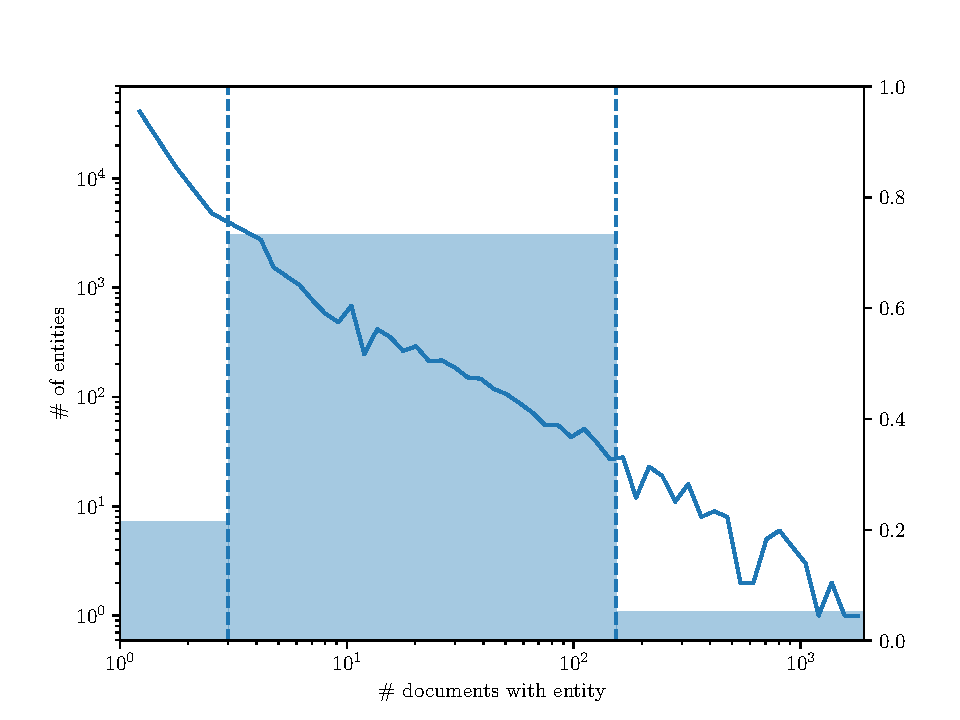
\includegraphics[width=0.8\textwidth]{figures/analysis/distribution}
  \caption[TAC KBP 2015 Query entity distribution]{\label{fig:kbpo:distribution}
    The solid line plots a histogram of how many documents a particular entity appeared in the TAC KBP 2016 corpus.
    The distribution is approximately a power-law distribution.
    Overlayed is a histogram of the frequency of the actual query entities used in the TAC KBP 2015 evaluation, binned by their frequency. We consider entities that appear in 3 or less unique documents (the 50th percentile) to be ``low'' frequency entities, those that appear more than 154 unique document (90th percentile) to be ``high'' frequency entities and those that appear in between to be ``medium'' frequency entities.
    The TAC KBP evaluation prefers medium frequency and low frequency entities.
  }
\end{figure}

\paragraph{The LDC query distribution and metrics.}
The first aspect we looked into was the distribution of entities that were queried in the official evaluations. 
The KBP evaluation is well known for using query entities that participate in several relations but are still not common enough to have a knowledge base entry on say Wikipedia.
We wanted to capture this property in our evaluation as well.

To get a better sense of the distribution of entities that were queried, we used the entities (i.e., people and organizations) that were recognized by the Stanford KBP entity linking system~\citet{stanford2017kbp} \pl{citep} and plotted a log-log distribution of the number of entities that appear in some number of documents (\reffig{kbpo:distribution}).
As one might expect, the distribution approximately follows a power-law and is extremely long-tailed: there are many entities that appear in just one or two documents. 

We then binned entities into three categories, ``low'' frequency entities that appear in at most 3 documents in the corpus (this is the 50th percentile), ``medium'' frequency entities that appear in between 3 and 154 (90th percentile) documents and finally, ``high'' frequency entities that appear in more than 154 documents.
The proportion of query entities in these three bins has been overlayed on top of the distribution in \reffig{kbpo:distribution}.
We see that a majority of the entities queried are medium frequency, followed by low frequency entities and a handful of high frequency entities.
We would like to ensure that our sampling distributions adequately capture these medium frequency entities. 

\begin{figure}
  \centering
  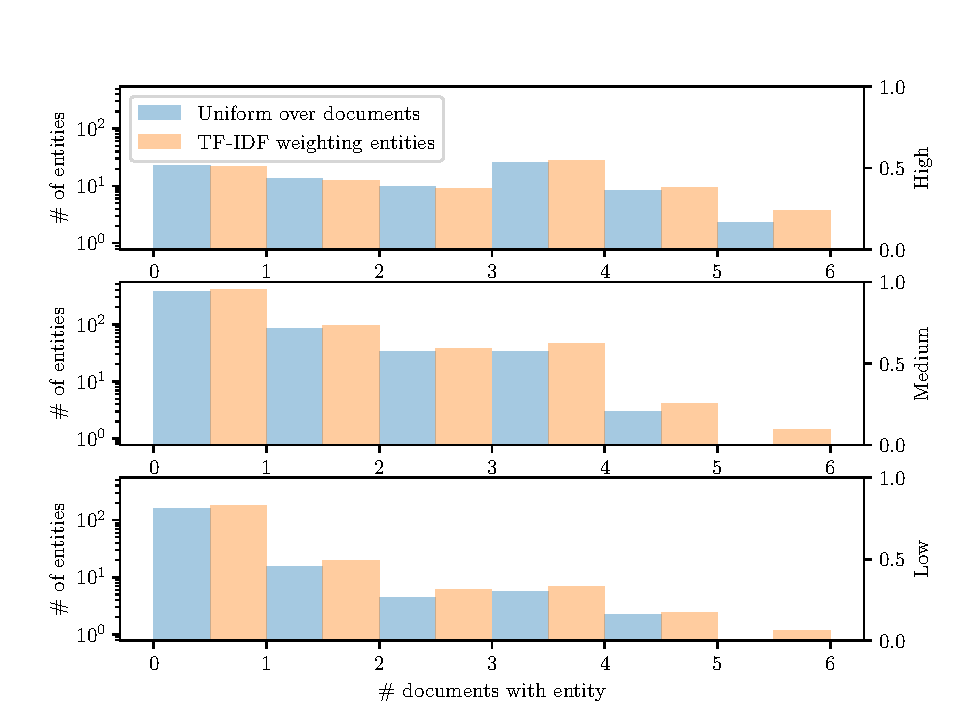
\includegraphics[width=0.8\textwidth]{figures/analysis/exhaustive_entity_cross}
  \caption[Comparison of document sampling distributions]{\label{fig:kbpo:exhaustive-entity}
  In order to properly test the entity linker when measuring recall, an important feature of KBP systems, we must identify documents for exhaustive annotation that contain some entity clusters.
  A sample of 200 documents uniformly picked from the document collection only exhibits clusters for high frequency entities.
  Our TF-IDF sampling scheme increases the frequency with which medium and low frequency entities appear across multiple documents in the sample.
  }
\end{figure}


\paragraph{Identifying diverse clustered documents.}
Next, we wanted to come up with a good distribution with which to query documents to exhaustively annotate.
It is not enough for us to ensure the documents contain a good distribution of medium frequency entities: we must also ensure that these entities appear in multiple documents to fairly test systems' entity linking components.

First, we tried using documents that were sampled uniformly from the corpus.
As \reffig{kbpo:exhaustive-entity} shows, 
a randomly sampled document contains a good range of low, medium and high frequency entities, but almost none of these entities are shared across the documents of the collection.
We note that the fact that low frequency entities dominate the entity distribution is to be expected because they constitute the majority of entities in any given document,\footnote{%
  We also tried sampling documents based on the frequency of entities they contained (estimated using the Stanford entity linker), but found that it did not significantly reduce the number of low frequency entities.} but we can correct for this when sampling relations.

Instead, we used a two-step sampling procedure.
First, we would \pl{remove modal} randomly sample documents for 20\% of our exhaustive document collection and then sample the remaining documents proportional to their aggregate TF-IDF scores with the entities identified in the first sample.
\reffig{kbpo:exhaustive-entity} shows the distribution of entities that were sampled by this method, using the Stanford entity linking system to identify entities in the first sample.
The method is able to increase the number of medium frequency entities appearing in multiple documents.
When implementing this method in practice, we explicitly avoided using the Stanford entity linking system when identifying entities in documents because we were concerned about the bias it would introduce into our recall estimates.
Instead, we identified the entities in the first sample using crowdsourcing with our exhaustive annotation interface.

\begin{figure}
  \centering
  \begin{subfigure}{0.7\textwidth}
    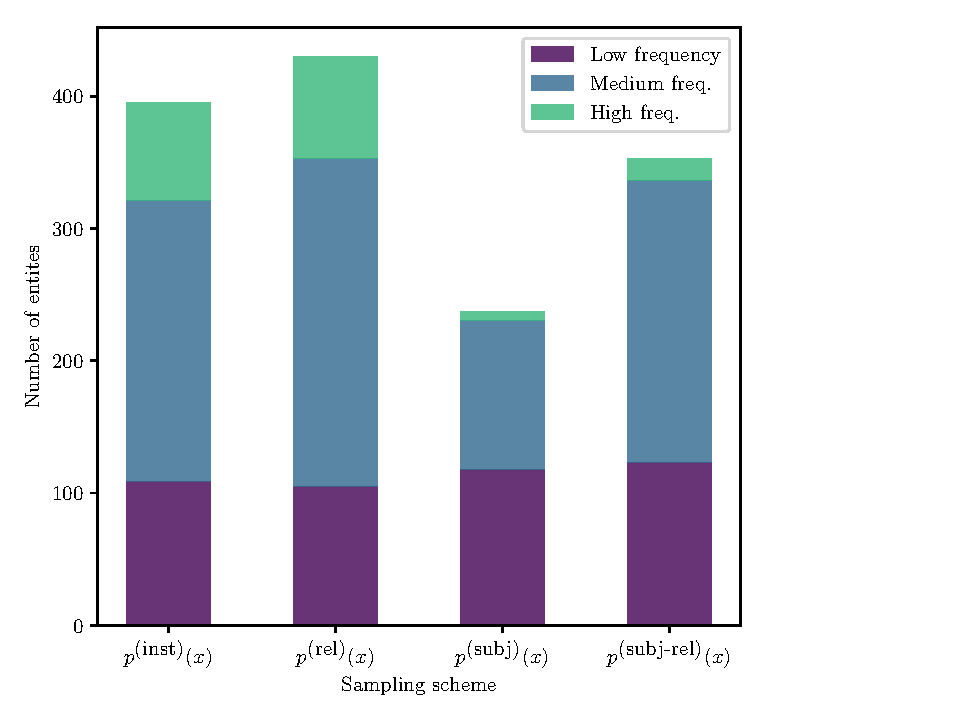
\includegraphics[width=\textwidth]{figures/analysis/selective_supervised_entity}
    \caption{\label{fig:kbpo:selective-supervised-entity} Distribution over entity classes}
  \end{subfigure}

  \begin{subfigure}{0.7\textwidth}
    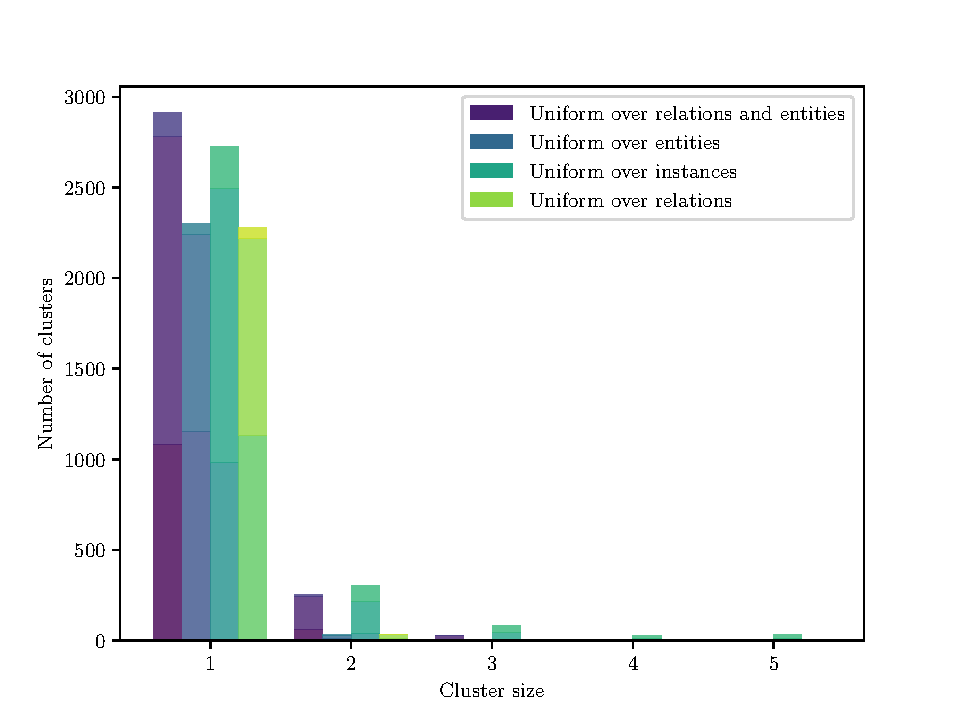
\includegraphics[width=\textwidth]{figures/analysis/selective_supervised_clusters}
    \caption{\label{fig:kbpo:selective-supervised-clusters} Distribution over entity clusters}
  \end{subfigure}

  \caption[Comparison of relation sampling schemes on their entity distributions]{\label{fig:kbpo:selective-supervised}
  We compared the types of entities that different relation instance sampling schemes preferred when we sampled 1,000 instances using them.
  Plots are averaged over 100 draws.
  (a) In terms of low, medium and high frequency entities, both $p^{\text{(subj)}}$ and $p^{\text{(subj-reln)}}$ sample fewer high frequency entities which are otherwise over represented.
  (b) In terms of how many entities were sampled with more than one relation (a cluster) were sampled, $p^{\text{(subj-reln)}}$ is still able to capture a comparable number of these unlike $p^{\text{(reln)}}$.
  }
\end{figure}

\begin{figure}
  \centering
  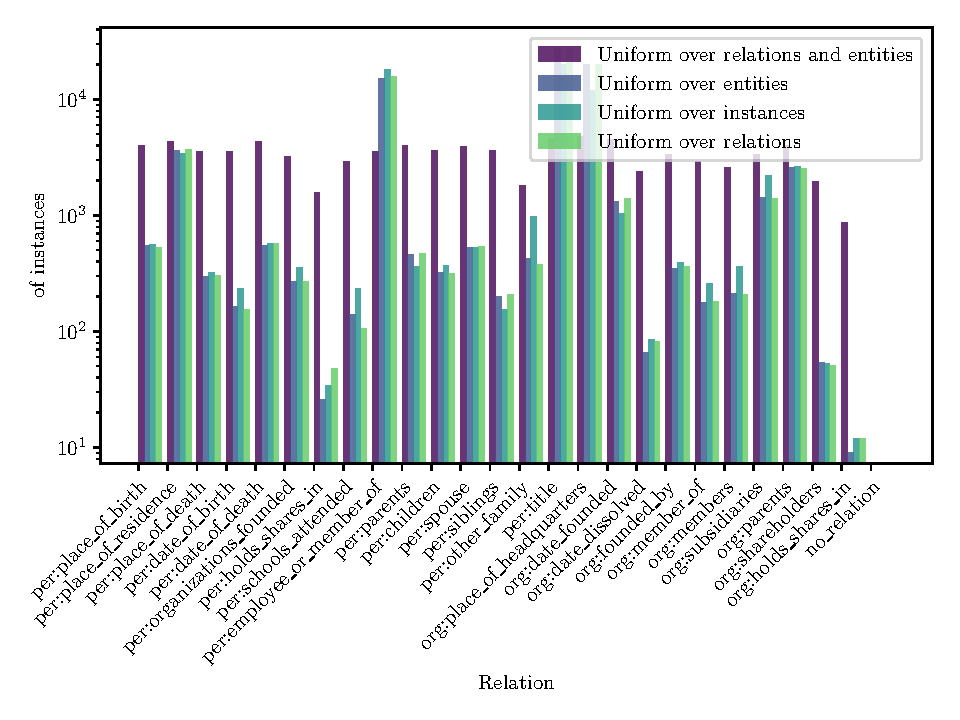
\includegraphics[width=0.9\textheight, angle=-90]{figures/analysis/selective_supervised_relations}
  \caption[Comparison of relation sampling schemes on their relation distributions]{\label{fig:kbpo:selective-supervised-relation}
  We compared the types of relations that different relation instance sampling schemes preferred when we sampled 1,000 instances using them.
  Plots are averaged over 100 draws.
  Both $p^{\text{(inst)}}$ and $p^{\text{(subj)}}$ do not draw any instances for particular relations, e.g.\ \texttt{org:shareholders}, while
  $p^{\text{(rel)}}$ and $p^{\text{(subj-rel)}}$ adequately represent each relation.
  }
\end{figure}

\paragraph{Identifying diverse clustered relations.}
Finally, we wanted to ensure that the entities we sampled from systems were well distributed both over medium frequency entities and over relations.
Unsurprisingly, the naive approach of uniformly sampling relations outputted by systems, is dominated by  high frequency entities (\reffig{kbpo:selective-supervised-entity}) on a few common relations (e.g., \texttt{per:title}; see \reffig{kbpo:selective-supervised-relation}).

Our first attempt at rectifying the problem was to use two distributions that sampled relations inversely proportional to the frequency of their subject entity and relation label respectively:
\begin{align*}
  p^{\text{(subj)}}(x) &\propto \frac{1}{|\texttt{subj}(x)|} &
  p^{\text{(rel)}}(x) &\propto \frac{1}{|\texttt{rel}(x)|}
\end{align*}
These distributions solved the two problems individually, but could not be combined because they differed in their support.
There was an additional problem: we hardly ever selected two relations from the same entity, as shown in \reffig{kbpo:selective-supervised-clusters}.
We wanted to maintain this property to be able to test the entity linking component of systems.

Our final proposed distribution rectified this by combining $p^{\text{(subj)}}(x)$ and $p^{\text{(rel)}}(x)$ and including a factor for the number of \textit{other} relations the subject entity had.
\begin{align*}
  p^{\text{(subj-rel)}}(x) &\propto \frac{|\texttt{subj-relns}(x)|}{|\texttt{subj}(x)| |\texttt{rel}(x)|},
\end{align*}
\reffig{kbpo:selective-supervised-entity} shows how this new distribution has both a better representation of medium frequency entities and is well balanced across all the relations.
\reffig{kbpo:selective-supervised-clusters} also shows that it is able to represent clusters of relatiosn with the same entity.

\subsection{Computing scores}

The official TAC KBP evaluation computes macro precision, recall and \fone{} using the average taken over all entities.
In the evaluation, systems are asked to present exactly one justification or provenance for every relation that is ultimately labeled by expert annotators.  
A relation is only judged correct if the entities in the relation are both correctly linked and entailed by the provided justification.
This specification presents a few problems and opportunities for our evaluation protocol that we discuss in this subsection. 

\paragraph{Utilizing multiple justifications for a relation.}
We would like systems to report multiple justifications for a particular relation to ensure that we can maximally reuse our annotations.
In principle, we only care if any of the reported justifications are correct.
However, we chose to measure the average correctness of all the justifications provided for two reasons:
  (a) first, we think that looking at average correctness gives a better indicator of system quality and 
  (b) it is hard to adapt a sampling based approach, which implicitly computes an average, to compute the ``maximum'' accuracy across all the justifications without having to annotate all the justifications.

\paragraph{Handling entity linking.}
When annotating a relation predicted by a system, we ask annotators to (a) ensure that the subject is correctly linked to a canonical entity within the document and (b) to attempt to link the entity to a Wikipedia page (as a globally canonical entity).
However, KBP systems often use their own entity linking scheme that does not correspond to the ones in Wikipedia.
As a result, we only handle entity linking \textit{within} a document, ensuring that the canonical entity span reported by the system corresponds to the one indicated by the annotators.
We hope to measuring cross-document entity linking in future work.

\paragraph{Factored scores}
\pl{put period consistently}
As part of our evaluation, we independently identify the correctness of the relation between the subject and object in the justification, as well as the correctness of the entity links of the subject and object.
As a result, we are able to compute correctness scores for relation classification, entity linking and the combined task.
Additionally, we are able to use per-relation and per-entity sampling distributions to report unbiased scores for each relation and entity category.
As a result, we are able to automate a basic error analysis method and make it more statistically sound.

\begin{figure}
  \centering
  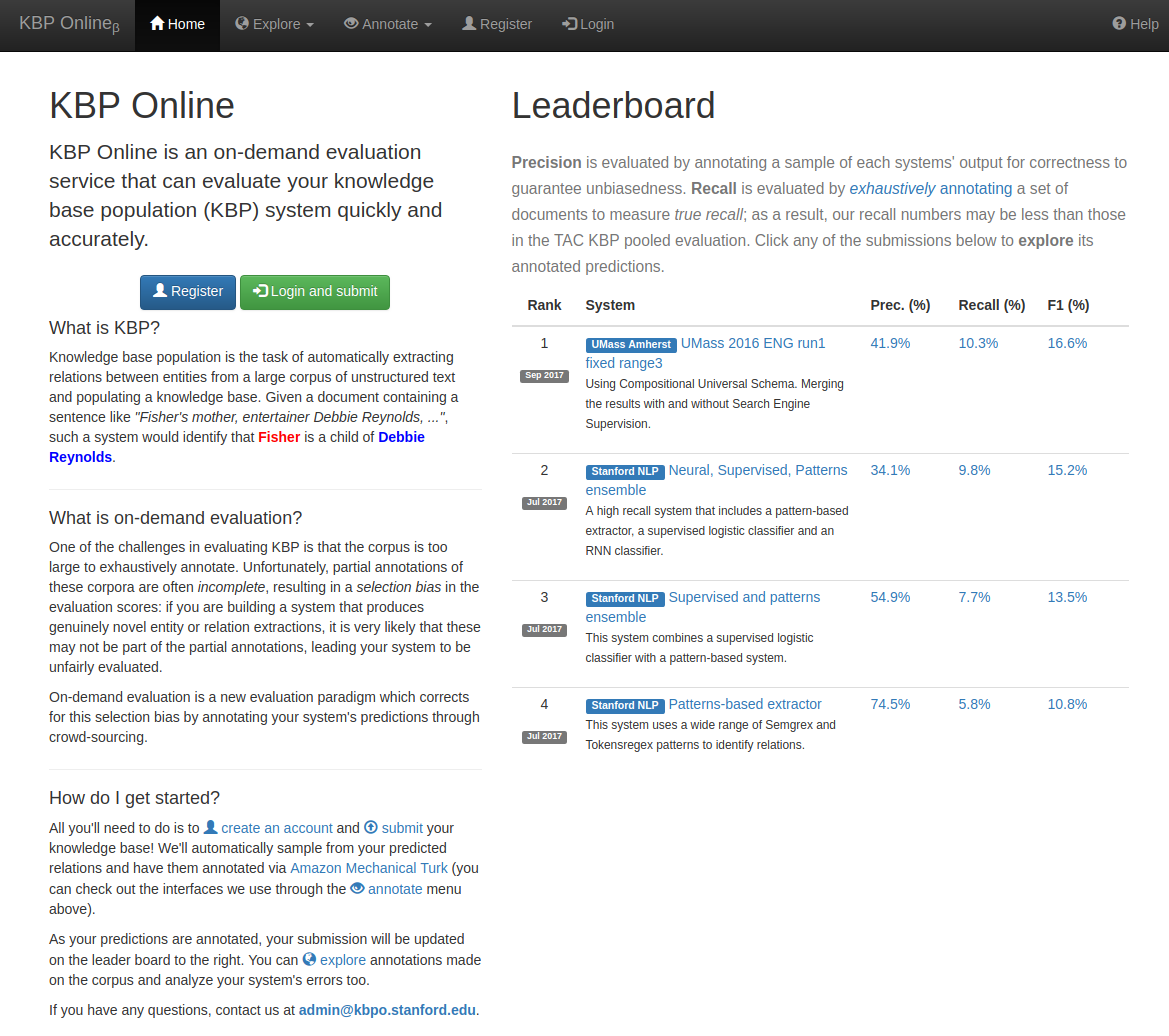
\includegraphics[width=\textwidth]{figures/interface/leaderboard}
  \caption[KBP Online]{\label{fig:kbpo:kbpo}
  A screenshot of the home page of our evaluation service, KBP Online.
  Our service takes care of the entire pipeline of sampling relation instances, annotating them and computing a score.
Once the system is completely evaluated, we show their entry on the home page leaderboard along with an 80\% confidence intervals estimated using bootstrap (not shown here).
  }
\end{figure}

\begin{figure}
  \centering
  \begin{subfigure}{0.7\textwidth}
    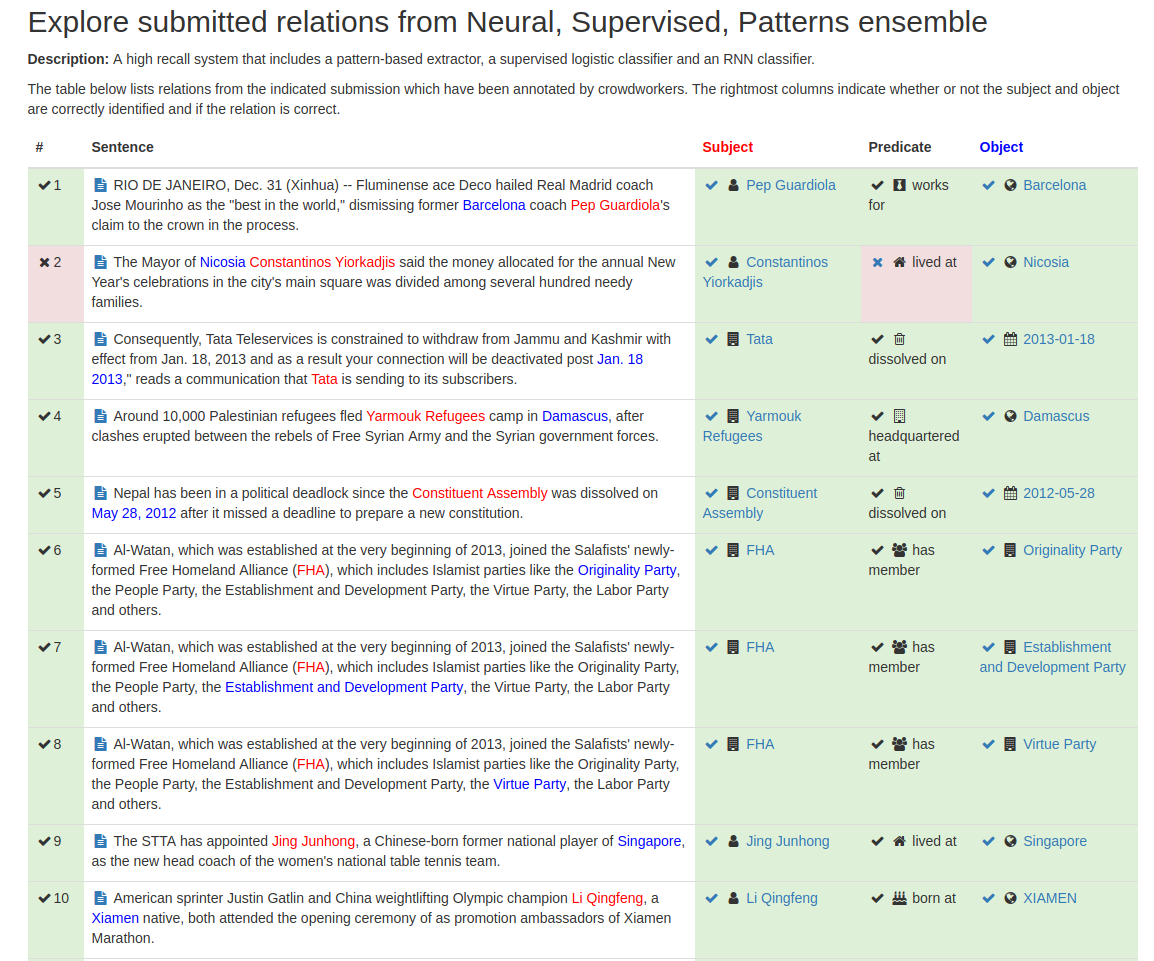
\includegraphics[width=\textwidth]{figures/interface/errors}
    \caption{\label{fig:kbpo:prediction-errors} Annotations of a particular system's predictions}
  \end{subfigure}

  \begin{subfigure}{0.7\textwidth}
    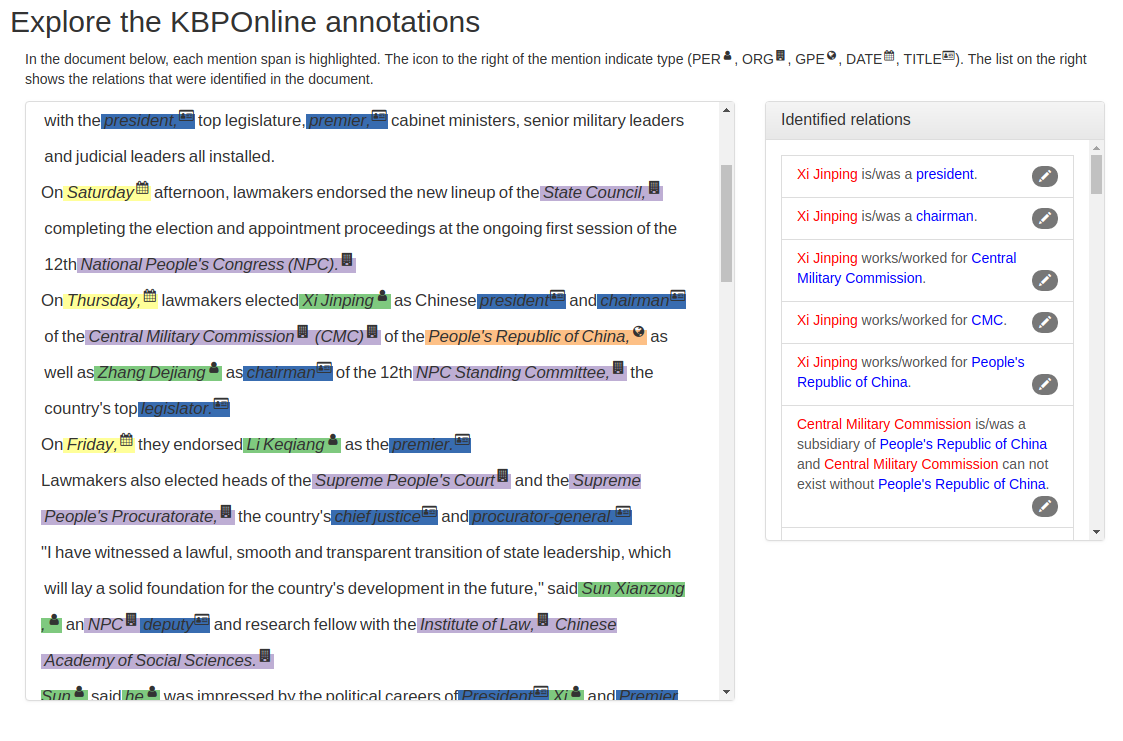
\includegraphics[width=\textwidth]{figures/interface/explore-data}
    \caption{\label{fig:kbpo:explore} Exhaustive annotations on entire documents}
  \end{subfigure}

  \caption[Features of KBP Online]{\label{fig:kbpo:kbpo-features}
  Apart from automating the evaluation of KBP systems, KBP Online also allows users to see (a) annotations of their predictions to identify the errors their systems have made and (b) annotations that were made on entire documents to identify relations that no system has been able to extract yet.
  }
\end{figure}

\subsection{Implementation details}
We implemented the online service using the Django web framework with Postgres as our relational database.
For performance reasons, we computed sampling distributions and evaluation scores entirely within the database.
We used the service to host the crowdsourcing interfaces described in \refsec{kbpo:application} and dynamically generated Human Intelligence Tasks (HITs) on Amazon Mechanical Turk from our server.
Maintaining exactly which relations were sampled and with what probability is important for our importance-reweighted estimator, and we stored these details in our database.
A large amount of effort went into automating the background tasks that collected annotations from Amazon Mechanical Turk, aggregated them and updating the scores.

In terms of an interface to users, they simply need to upload a single file in the official TAC KBP format containing their predicted knowledge base.
Our service entirely takes care of computing the required statistics and sampling from the systems.
At present, we collect about 500 samples for every system, which corresponds to an 80\% confidence interval of $\pm 3\%$.
Once the system is completely evaluated, we show the entry on the home page leaderboard (\reffig{kbpo:kbpo}) along with an 80\% confidence intervals estimated using bootstrap (not shown here).

Additionally, we allow users to drill down into annotations we collected on documents and on a system's predictions (\reffig{kbpo:kbpo-features}).
These annotations help users identify the errors systems are making as well as identify relations that no system is currently able to extract.
We hope to include a feature that also provides a quantitative summary of the models performance on different relations and break down errors between relation classification and entity linking.
We hope that these features will help push the state of the art of knowledge base population forward.

